\documentclass[11pt]{article}
\usepackage[margin=1in]{geometry}
\usepackage[T1]{fontenc}
\usepackage{mathptmx}
\usepackage[scaled=.92]{helvet}
\usepackage{courier}
\usepackage{amsmath,amssymb}
\usepackage{booktabs,multirow}
\usepackage{graphicx}
\usepackage{xcolor}
\usepackage{caption}
\usepackage{subcaption}
\usepackage{enumitem}
\usepackage{algorithm}
\usepackage{algpseudocode}
\usepackage{tikz}
\usetikzlibrary{positioning,arrows.meta,fit,backgrounds,calc}
\usepackage[numbers,sort&compress]{natbib}
\usepackage{microtype}
\usepackage[colorlinks=true,linkcolor=blue!50!black,citecolor=blue!50!black,urlcolor=blue!50!black]{hyperref}

\captionsetup{font=small,labelfont=bf}
\renewcommand{\topfraction}{.9}\renewcommand{\bottomfraction}{.6}\renewcommand{\textfraction}{.1}\renewcommand{\floatpagefraction}{.75}\setcounter{topnumber}{3}\setcounter{totalnumber}{5}
\setlist{itemsep=2pt,topsep=4pt}
\newcommand{\tn}[1]{\texttt{#1}}
\newcommand{\RQ}[1]{\textbf{RQ#1}}

\title{\textbf{Reading the Architecture off the Weights:\\ Manifest-Only Recovery of Neural Network Anatomy,\\ with an Interactive Explorer}}
\author{Sattaya Singkul\\ Researcher\\ \texttt{joeysattaya@gmail.com}}
\date{}

\begin{document}
\maketitle

\begin{abstract}
To decide whether a model fits a device, how to quantize it, or simply what it is, practitioners need its architecture: which blocks repeat, what each block computes, how the components connect, and where the parameters sit. This information is scattered across model cards, family-specific configuration schemas and modeling code that must be read or executed. We show that most of it is already present in a much smaller artifact that almost every public checkpoint exposes: the \emph{tensor manifest}, the list of tensor names, shapes and storage types that a safetensors file keeps in a header of a few tens of kilobytes. We present a method that turns a manifest into a structured anatomy. It normalizes quantized storage to logical tensors, finds repeated blocks in the module tree and types them by structural signature, assigns roles to the regions of each block from the algebra of their shapes, links components by matching residual widths, and finally fuses the fields that shapes cannot determine from \tn{config.json} while checking that file against the weights. On 511 architectures instantiated from the \tn{transformers} library, with ground truth taken from module classes the method never sees, per-tensor role accuracy is 96.4\% (macro over architectures) against 69.2\% for name-pattern rules, and 94.7\% when every name is replaced by a random token. Logical parameter counts are exact for all models, also under NVFP4, FP8 and GPTQ storage. Shapes alone recover head geometry for about 72\% of models; with configuration fusion this rises to 96\%, and the consistency check finds that 95\% of configurations agree with their weights, the rest being attention variants whose fields mean something else. The method runs in about 13\,ms per model in a browser. We release it as an open, bilingual explorer that reads any Hugging Face repository over HTTP range requests, and we illustrate it on nine 2026 models, including a 121B hybrid Mamba--MoE vision-language model, two speech transducers and a video diffusion transformer.
\end{abstract}

\section{Introduction}

A deployment engineer handed a new checkpoint asks the same questions every time. How many layers are there, and are they all alike? Is it a mixture of experts, and how much of the size is experts? Which part runs once per input and which part runs once per generated token? Where will 4-bit quantization hurt first? For a familiar family, \tn{config.json} answers these questions. For anything new it often does not. Configuration keys differ across families (\tn{hidden\_size}, \tn{d\_model}, \tn{n\_embd}); composite models nest several schemas; and fields such as \tn{layers\_block\_type} only make sense after reading the modeling code. Reading that code is slow, and running it with \tn{trust\_remote\_code} is a known supply-chain risk on public hubs~\citep{zhao2024modelsarecodes}. Graph viewers such as Netron~\citep{netron} or Model Explorer~\citep{modelexplorer2024} need an exported graph and, in practice, the whole file.

A smaller artifact is almost always available. A safetensors file~\citep{safetensors} begins with an 8-byte length and a JSON header listing every tensor's name, dtype, shape and byte offsets. Two HTTP range requests fetch it. Across the 511 architectures studied here its median size is 47\,KB, about $6\times10^{-5}$ of the weights in BF16 (Figure~\ref{fig:cost}). PyTorch zip checkpoints carry the same facts in their \tn{data.pkl} record, which can be read without touching tensor data.

This paper asks a simple question: \emph{how much of a model's architecture can be read from its manifest alone, and how reliably?} The question matters in practice, because a tool that answers it can explain any hub model in a browser tab before anyone downloads it. It also has an analytical side. Some properties of an architecture leave no trace in tensor shapes, and an honest tool should say which ones, measure how often a prior gets them right, and fill them from a better source when one exists.

Our starting observation is that a manifest carries two kinds of evidence that complement each other. The \emph{name tree} reveals structure: integer-indexed lists are stacks of blocks, identical subtrees are identical block types, and the module that owns a stack delimits a component. The \emph{shapes} reveal function: every block shares a residual width $d$; an attention region is a set of projections that leave $d$ and one that returns to it; a mixture of experts is a set of tensors whose leading dimension equals the output size of a router; a selective state-space mixer is a depthwise convolution next to a handful of per-head vectors; and two components are connected where the output width of one equals the input width of another. Names help break ties, but as we show, most of the work survives when every name is replaced by a random token.

\paragraph{Contributions.}
\begin{itemize}
\item We formulate \emph{manifest-only architecture recovery}, define an anatomy representation that is useful to people (components and data path, stacks and block types, regions and roles, logical sizes), and analyse which properties are not identifiable from shapes (\S\ref{sec:problem}).
\item We give a recovery algorithm that combines module-tree structure with shape algebra and width matching, normalizes six quantized storage layouts, and fuses non-identifiable fields from \tn{config.json} while checking the configuration against the weights (\S\ref{sec:system}, \S\ref{sec:method}).
\item We build an open, bilingual explorer around the algorithm that reads any Hugging Face repository by range requests, shows every value with its provenance, and walks users through a model part by part (\S\ref{sec:tool}).
\item We construct a benchmark of 511 architectures with exact manifests and independent ground truth, and answer five research questions on role recovery, structure, robustness, identifiability and cost (\S\ref{sec:setup}, \S\ref{sec:results}). Case studies on nine 2026 models illustrate the coverage (\S\ref{sec:cases}).
\end{itemize}

\section{Background and related work}
\label{sec:related}

\paragraph{How checkpoints describe themselves.} A modern checkpoint usually ships three descriptions of the same model: the weights, a configuration file, and code. Model cards~\citep{mitchell2019modelcards} add a human-written summary whose architectural fields are free text. The configuration is authoritative for the library that wrote it, but its schema is family-specific, and for new families it must be interpreted through code. Pickle-based weight formats can execute code on load~\citep{zhao2024modelsarecodes}; safetensors avoids this, and its header is the most uniform description that exists across families.

\paragraph{Model visualization.} Netron~\citep{netron}, TensorBoard and Model Explorer~\citep{modelexplorer2024} render operator graphs from exported formats. They show what is in a graph faithfully but do not group operators into semantic parts, and they need the file. Transformer Explainer~\citep{cho2024transformerexplainer} explains one fixed architecture interactively and very well. Our explorer sits between these: semantic parts for arbitrary architectures, from a few kilobytes, with an explanatory walk-through borrowed from the second line of work.

\paragraph{Architecture inference.} Side-channel attacks recover architectures from the cache timing or memory traces of a running model~\citep{yan2020cachetelepathy,hu2020deepsniffer}. There the observer lacks the file; here the header is public and the difficulty is interpretation. Weight-based fingerprinting such as HuRef~\citep{zeng2024huref} identifies a model's lineage from weight values; we never read values.

\paragraph{Architectures and storage formats.} Our rules encode the shape signatures of attention and its variants (grouped-query~\citep{ainslie2023gqa} and latent attention~\citep{deepseekv2}), sparse mixtures of experts~\citep{shazeer2017moe,fedus2022switch}, selective state-space and linear-attention mixers~\citep{gu2023mamba,dao2024mamba2,yang2025gateddeltanet} and their hybrids~\citep{nemotronh2025}, conformers~\citep{gulati2020conformer,rekesh2023fastconformer}, transducers~\citep{graves2012rnnt,xu2023tdt}, diffusion transformers~\citep{peebles2023dit} and tabular in-context learners~\citep{hollmann2025tabpfn,qu2025tabicl}. For storage we handle GPTQ~\citep{frantar2023gptq}, AWQ~\citep{lin2024awq}, FP8~\citep{micikevicius2022fp8}, MXFP4~\citep{rouhani2023mx}, NVFP4~\citep{nvidia2025nvfp4} and MLX layouts.

\section{Problem formulation}
\label{sec:problem}

\subsection{Manifests and anatomies}
A manifest is a set $\mathcal{M}=\{(n_i, s_i, \tau_i)\}$ of tensor names (dot-separated paths), shapes and storage dtypes. Optionally a configuration $\mathcal{C}$, a nested key--value tree, is also available. We want an \emph{anatomy} $\mathcal{A}$ consisting of:
\begin{itemize}
\item \textbf{components} (for example a vision tower, a projector, a language backbone, a prediction network), each with a residual width $d$, a modality and a role, and directed \textbf{edges} for the data path;
\item within each component, \textbf{stacks} of repeated blocks, each block assigned a \textbf{block type};
\item within each block type, \textbf{regions} labeled with a role from a fixed taxonomy: attention, cross-attention, feed-forward, mixture of experts, SSM or linear attention, convolution module, adaLN modulation, recurrent cell and norm; and outside blocks, input stem, output head and adapter;
\item per-tensor roles (query, router, expert, \dots), logical shapes under quantized storage, and derived quantities such as parameters, stored bytes, KV-cache bytes per token and active parameters per token;
\item for every architectural field, its \textbf{provenance}: measured from the manifest, read from $\mathcal{C}$ and checked against the manifest, or estimated.
\end{itemize}

\subsection{What a manifest cannot identify}
\label{sec:ident}
Several properties leave no trace in shapes.
(i) \emph{Head count versus head size.} A projection $W_q\in\mathbb{R}^{Hh\times d}$ with $H$ heads of size $h$ has the same shape as one with $H/2$ heads of size $2h$. The pair is identifiable only through per-head parameters, such as query and key norms of width $h$ or relative-position biases of shape $H\times h$; otherwise only the product $Hh$ and the ratio of query to key--value width are.
(ii) \emph{Masking.} A decoder-only language model with tied embeddings stores exactly the tensors of a bidirectional encoder of the same size.
(iii) \emph{Routing and activation.} The number of experts is visible; the number used per token is not. Gated and ungated feed-forwards differ in matrix count, but SiLU and GELU do not.
(iv) \emph{Order inside a block.} Pre-norm and post-norm blocks have identical tensors.

These limits shape the design. The recovery algorithm reports such fields only as estimates, the explorer labels them as such, and when a configuration is available the fields are read from it and the configuration is checked against the shapes (\S\ref{sec:fusion}). The evaluation measures both how often the estimate is right and how much fusion adds.

\section{System overview}
\label{sec:system}

\begin{figure}[t]
\centering
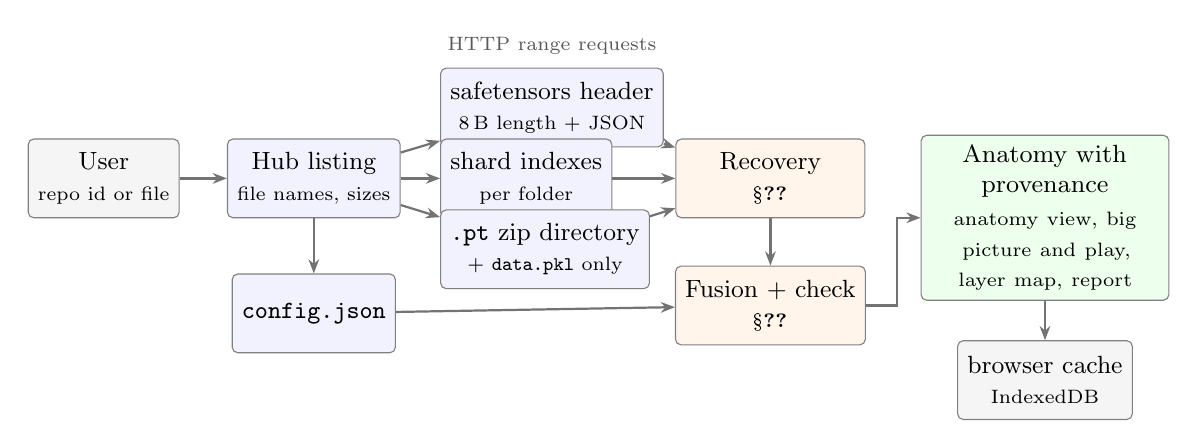
\begin{tikzpicture}[font=\small, node distance=4mm and 5mm,
  b/.style={draw=black!50, rounded corners=2pt, align=center, inner sep=3.5pt, minimum height=10mm, fill=#1},
  b/.default=white, arr/.style={-{Stealth[length=1.8mm]}, thick, black!55}, lab/.style={font=\scriptsize, black!65}]
\node[b=black!4] (u) {User\\ \scriptsize repo id or file};
\node[b=blue!5, right=6mm of u] (api) {Hub listing\\ \scriptsize file names, sizes};
\node[b=blue!5, right=of api, yshift=9mm] (st) {safetensors header\\ \scriptsize 8\,B length + JSON};
\node[b=blue!5, right=of api] (ix) {shard indexes\\ \scriptsize per folder};
\node[b=blue!5, right=of api, yshift=-9mm] (pt) {\tn{.pt} zip directory\\ \scriptsize + \tn{data.pkl} only};
\node[b=blue!5, below=7mm of api] (cf) {\tn{config.json}};
\node[b=orange!8, right=8mm of ix, minimum width=24mm] (inf) {Recovery\\ \scriptsize \S\ref{sec:method}};
\node[b=orange!8, below=6mm of inf] (fz) {Fusion + check\\ \scriptsize \S\ref{sec:fusion}};
\node[b=green!7, right=7mm of inf, yshift=-5mm, text width=29mm] (v) {Anatomy with provenance\\[1pt]\scriptsize anatomy view, big picture and play, layer map, report};
\node[b=black!4, below=5mm of v] (db) {browser cache\\ \scriptsize IndexedDB};
\draw[arr] (u) -- (api); \draw[arr] (api) -- (st); \draw[arr] (api) -- (ix); \draw[arr] (api) -- (pt); \draw[arr] (api) -- (cf);
\draw[arr] (st) -- (inf); \draw[arr] (ix) -- (inf); \draw[arr] (pt) -- (inf); \draw[arr] (inf) -- (fz); \draw[arr] (cf) -- (fz);
\draw[arr] (fz.east) -- ++(4mm,0) |- (v.west); \draw[arr] (v) -- (db);
\node[lab, above=0.5mm of st] {HTTP range requests};
\end{tikzpicture}
\caption{End-to-end workflow. Only descriptive bytes are fetched: the file listing, safetensors headers, shard indexes, the zip directory and pickle record of PyTorch checkpoints, and the configuration. Recovery and fusion run in the browser; results are cached locally so that a returning visitor does not repeat them.}
\label{fig:workflow}
\end{figure}

Figure~\ref{fig:workflow} shows the workflow. Given a repository id, the explorer lists the repository and decides what describes the weights. Safetensors files are preferred; their shard indexes are read per folder, so that a diffusers-style repository with \tn{transformer/}, \tn{text\_encoder/} and \tn{vae/} folders yields one prefix per component. For each safetensors file two range requests fetch the length and the header. If a repository has only PyTorch zip checkpoints, the reader fetches the last 64\,KB of the file to locate the zip central directory, then fetches only the \tn{data.pkl} record and interprets it with a restricted unpickler that rebuilds names, shapes and dtypes and never resolves a Python callable. The configuration is fetched alongside. Progress is shown at each step (``reading header 3 of 12, 41\,KB so far''), and the analysed result is cached in the browser.

The manifest then passes through the recovery algorithm of \S\ref{sec:method}, and the result through configuration fusion. Every field of the final anatomy carries its provenance, which the interface displays next to the value.

\section{Recovering the anatomy}
\label{sec:method}

Every rule in this section reads only shapes, dtypes and the structure of the name tree. A small lexicon of name fragments (\tn{attn}, \tn{mlp}, \tn{experts}, \dots) is consulted to break ties that shapes leave open and can be switched off; \S\ref{sec:results} measures the method with and without it. Algorithm~\ref{alg:main} summarizes the procedure.

\begin{algorithm}[t]
\caption{Manifest-only anatomy recovery with configuration fusion}
\label{alg:main}
\small
\begin{algorithmic}[1]
\Require manifest $\mathcal{M}$, optional configuration $\mathcal{C}$
\State $\mathcal{T}\gets$ \Call{Normalize}{$\mathcal{M}$} \Comment{logical shapes, stored bytes}
\State build the module tree; find lists, expert lists, sub-layer lists, block lists, homes
\ForAll{block list $L$}
  \State group items by structural signature into block types; record the type sequence
  \ForAll{block type $\beta$}
    \State $d\gets$ width of the leaf norms of a representative block
    \State classify children by shape rules; split nested blocks; pair halves; test transposition
  \EndFor
\EndFor
\State label stems and heads; detect adapters, transducer joints, timestep MLPs, message passing
\State choose the backbone and family; derive $d$, $L$, $f$, $E$, $V$, KV bytes per token
\If{$\mathcal{C}$ is given}
  \State match sub-configurations to components by width and depth; read $H$, $H_{kv}$, $h$, top-$k$
  \State check $Hh=x$ and $H_{kv}h=x_{kv}$; label each field \emph{config} or report the mismatch
\EndIf
\State \Return anatomy with provenance and an evidence string for every decision
\end{algorithmic}
\end{algorithm}

\subsection{Normalizing storage}
Quantized checkpoints store one logical weight as several tensors. We group tensors by module and recognize the layout by dtype and shape before looking at names. NVFP4 stores a \tn{U8} tensor of shape $[o, i/2]$, an FP8 scale tensor $[o, i/16]$ and a scalar second-level scale; the logical shape is $[o, i]$ and the group size follows from the ratio. FP8 stores an FP8 weight with a scalar, per-channel $[o,1]$ or block scale. GPTQ stores \tn{qweight} as \tn{I32} $[i/8, o]$ with scales $[i/g, o]$; AWQ packs the other axis, and the two are told apart by which axis the scales share. MXFP4 and MLX layouts follow the same pattern. Auxiliary tensors count toward stored bytes but not toward parameters.

\subsection{Blocks from the module tree}
Names form a tree. A node whose children are all integers, or keys such as \tn{expert\_0}, \tn{expert\_1}, \dots, is a \emph{list}. An item is \emph{composite} if its subtree holds at least two parameterized modules; this separates blocks from \tn{nn.Sequential} wrappers around single layers.

\emph{Expert lists} are lists nested inside the item of another list whose items are structurally identical two- or three-matrix MLPs without norms, usually beside a router whose first dimension equals the number of items. Stacked experts instead appear as 3-D tensors $[E, \cdot, \cdot]$ with one trailing dimension equal to the block width.

\emph{Block lists} are the innermost composite lists that are not expert lists, with one correction: when every item of an outer list holds one or more short inner lists of equal length (T5's \tn{block.$i$.layer.$j$}, or LongCat's two attention and two MLP sub-layers per layer), the inner items are sub-layers and the outer items are the blocks.

Each block list belongs to a \emph{home}, the module that owns it, raised through its ancestors while no other stack lives there and, in multi-folder repositories, never above the folder. Homes become components, so embeddings and heads next to an \tn{encoder} wrapper join the right component. Inside a list, each block receives a signature: the sorted multiset of pairs (relative path with indices masked, tensor rank). Identical signatures form a block type. In a hybrid stack such as Nemotron-H~\citep{nemotronh2025} this yields one type for each of Mamba-2, MoE and attention layers, and the sequence of types is the layer pattern.

\subsection{Regions by shape algebra}
For each block type we analyse one representative block. Its residual width $d$ is the length of the vectors held by its leaf norm modules; this is more robust than counting matrix dimensions, which an SSM's inner width can dominate. The children of the block are then classified. Let a matrix be an \emph{input} if its second dimension is $d$ and an \emph{output} if its first dimension is $d$.

\begin{itemize}
\item \textbf{Mixture of experts:} stacked 3-D experts or an expert list, with a router $[E', d]$ where $E\le E'\le E+8$ (some routers reserve extra slots).
\item \textbf{SSM / linear attention:} a depthwise convolution $[C,1,k]$ with $k\le 8$ plus recurrence parameters attached directly to the mixer: at least two vectors of a common length $n_h\neq d$ (for $A$, $D$, the $\Delta t$ bias), or a 2-D or 3-D state tensor with a small last dimension. Mixers without a convolution (xLSTM, RWKV) are recognized by two or more per-head gate projections $[\le 64, d]$ or by decay vectors.
\item \textbf{Feed-forward:} one output $[d,f]$ and one or two inputs $[f,d]$, or one fused input $[2f,d]$ with $f>1.3d$.
\item \textbf{Attention:} one output $[d,x]$ with one or more inputs, or one fused input $[x+2x_{kv}, d]$. Inputs whose own input width is produced inside the region are internal; this keeps the low-rank chains of latent attention~\citep{deepseekv2} inside one region. A region whose external inputs include $d$ and at least two projections from another width $w\ge128$ is \emph{cross-attention} from the component of width $w$. Vectors in norm-only submodules whose length divides $x$ give the head size; parameters of shape $[H,h]$ with $Hh=x$ give both factors.
\item \textbf{Recurrent cell:} two or more matrices whose rows are $3h$ or $4h$ (GRU, LSTM), none returning to $d$.
\item \textbf{Convolution module:} a depthwise convolution with pointwise $[C,C',1]$ convolutions or batch-norm statistics.
\item \textbf{adaLN modulation:} a single matrix $[kd, t]$ from a width $t<d$, or $k\in\{6,9,12,18\}$ when $t=d$, or a $[1,k,d]$ scale--shift table.
\end{itemize}

Three refinements matter in practice. A child holding two non-leaf sub-modules that classify into different confident roles (an attention and an MLP inside one ``inducing block'') is split. Two half feed-forwards in sibling modules ($[f,d]$ in \tn{intermediate} and $[d,f]$ in \tn{output}) are paired. If a region is weak in the usual layout but becomes attention when every matrix is transposed, the weights are stored as $[\text{in},\text{out}]$, as GPT-2's \tn{Conv1D} does.

\subsection{Stems, heads and the data path}
Outside blocks, a matrix $[V,d]$ with $V>d$ is a token table and its twin an untied output head; a vector of length $V$ is the head's bias; a small table beside a token table or convolutional stem is a position or type embedding. A matrix chain whose free input width equals one component's width $d_X$, or $k^2 d_X$ for $k\in\{2,3,4\}$ after pixel shuffling, and whose free output width equals another component's $d_Y$, becomes an \emph{adapter} with edges $X\to\text{adapter}\to Y$.

Three further patterns become components of their own. A \emph{transducer} has a label embedding $[V, h_p]$ next to a recurrent cell, an encoder projection $[j, d_{\text{enc}}]$, and an output $[V', j]$ with $V\le V'\le V+16$; the excess $V'-V$ is the number of duration bins of a token-and-duration transducer~\citep{xu2023tdt}. A \emph{diffusion denoiser} has a timestep MLP from a sinusoidal width (128, 256 or 320) to a width $t$ that feeds the modulation matrices in its blocks. A group of square maps $[C,C]$ with an aggregation matrix $[C, rC]$ is a message-passing layer with $r$ reducers.

The backbone is the largest component that owns a token table or output head. The family (decoder, prefix LM, encoder--decoder, transducer, diffusion denoiser, encoder) follows from the components and edges.

\subsection{Configuration fusion and consistency checking}
\label{sec:fusion}
When a configuration is available, the fields of \S\ref{sec:ident} are read from it. Configurations of composite models nest several sub-configurations, so we first decide which sub-configuration describes which component. Every object node of $\mathcal{C}$ that declares a width (\tn{hidden\_size}, \tn{d\_model}, \tn{n\_embd}, \tn{dim}, \dots) is a candidate; a component is matched to the candidate whose width equals its residual width, preferring one whose layer count equals the component's and whose path names the right kind of component (\tn{text}, \tn{llm}, \tn{vision}, \tn{audio}). From the match we read the head count, key--value head count, head size and routing top-$k$.

The match is then checked against the weights: the product of head count and head size must equal the width $x$ of the attention projections, and the key--value product must equal $x_{kv}$. A field that passes is labeled \emph{config}; a disagreement is reported rather than resolved, because it usually means that a field carries a different meaning in that family (\S\ref{sec:rq4}). Without a configuration, the head size falls back to a prior (128 for $d\ge2048$, otherwise 64) and is labeled \emph{estimate}.

\subsection{Derived quantities and cost}
Parameters and stored bytes are sums over logical and stored tensors. KV-cache bytes per token are $2\sum_{\ell\in\text{attn}} x_{kv}^{(\ell)}\, b$; SSM layers keep a constant state instead. With a top-$k$ value, active parameters per token are the non-expert parameters plus $k/E$ of the experts. The procedure makes a few passes over the tree and is near-linear in the number of tensors.



\section{The interactive explorer}
\label{sec:tool}

The algorithm is the core of an open web tool~\citep{singkul2026explorer}. We built it for a hands-on workshop on edge inference, where participants had to understand a speech model before compressing it, and then generalized it to any architecture.

\paragraph{Design goals.} Three goals guided the interface. First, \emph{answer the first question in one screen}: what the model is made of and how big each part is. Second, \emph{show where each value comes from}, so that a reader can distinguish a measurement from a configuration value and from an estimate. Third, \emph{explain by walking}, letting a newcomer step through the model from input to output, seeing what each part receives and produces, instead of watching every layer animate.

\begin{figure}[t]
\centering
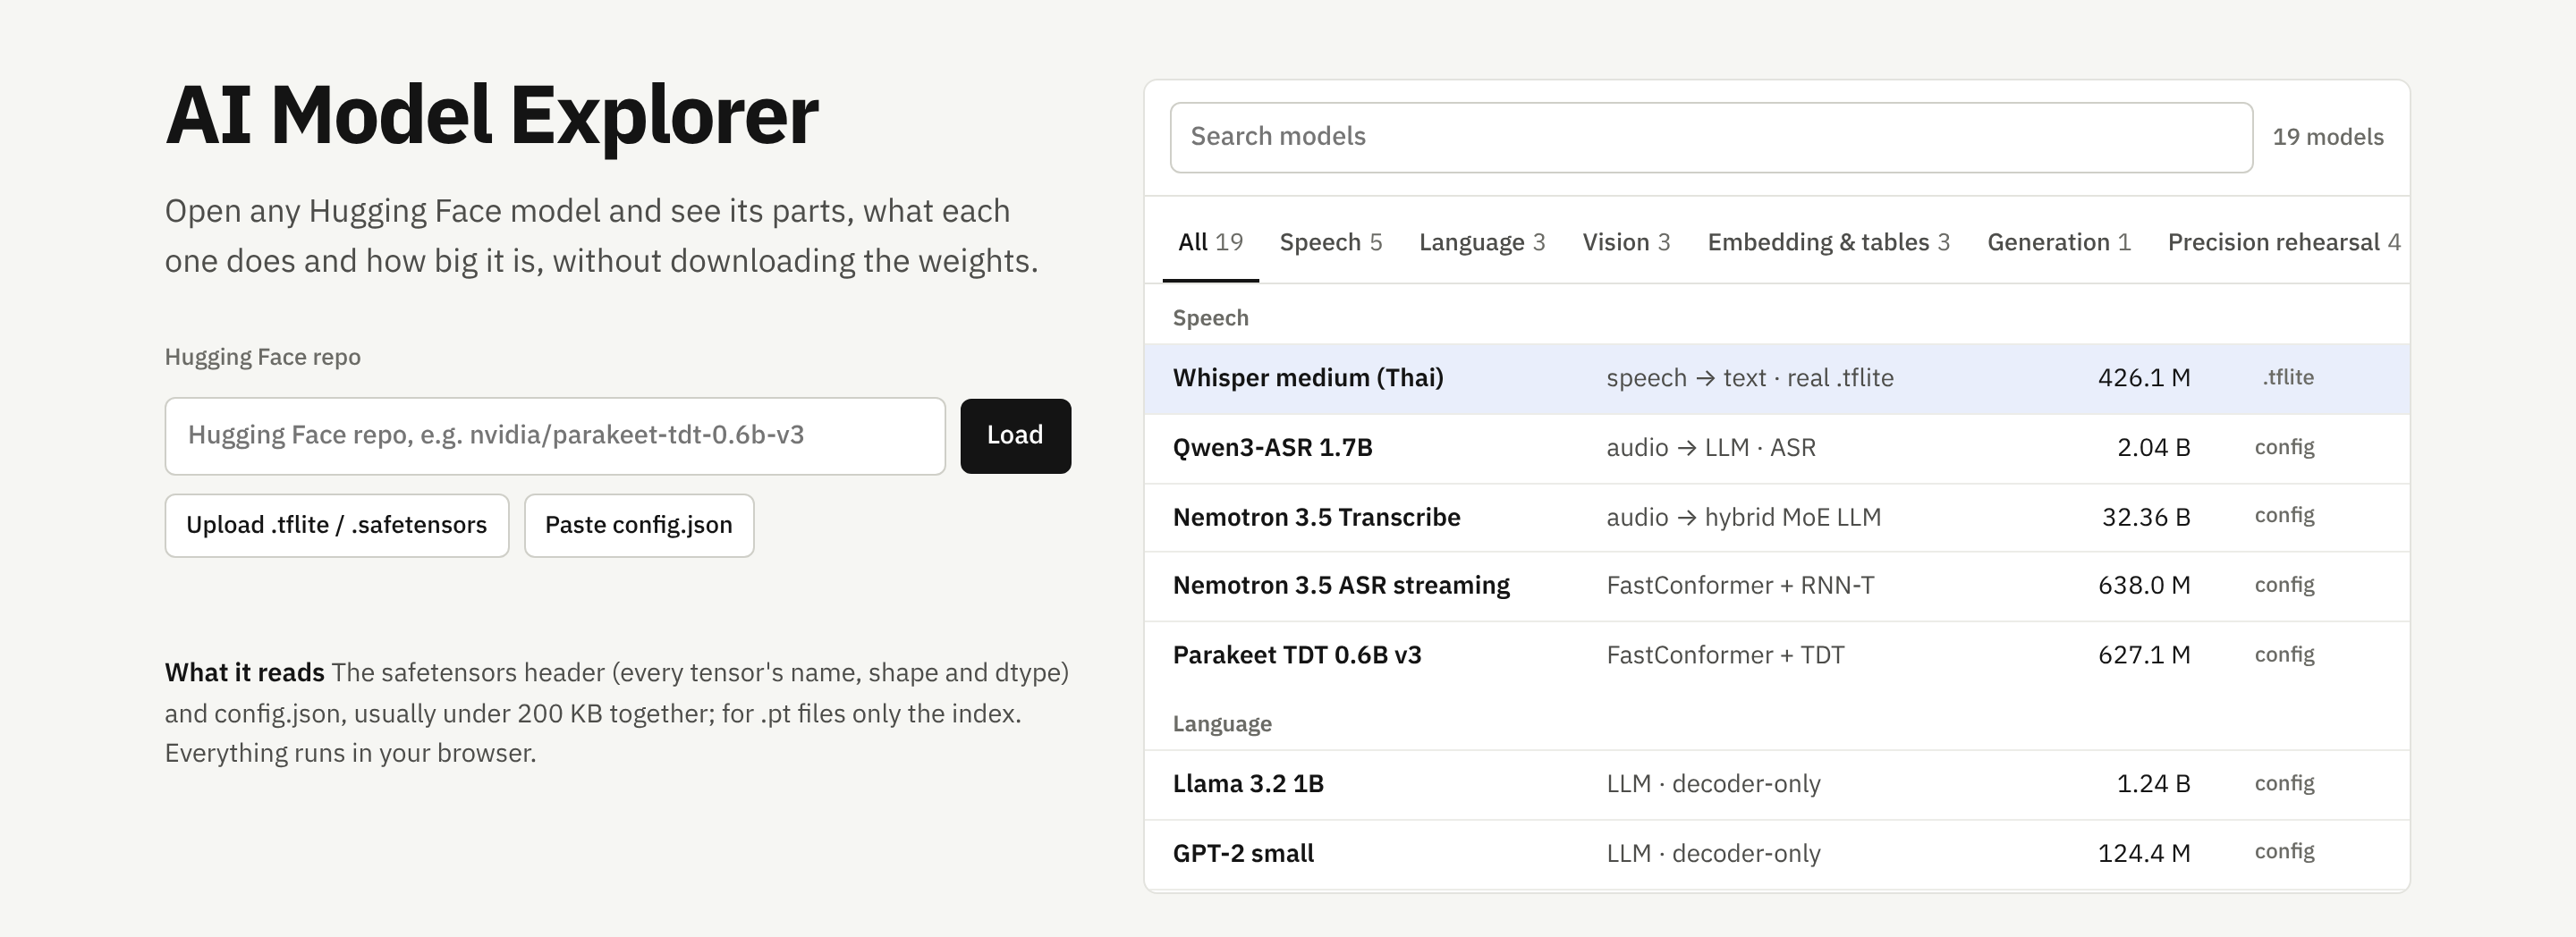
\includegraphics[width=\linewidth]{fig/ui_library.png}
\caption{Entry screen. A repository id, an uploaded \tn{.safetensors} or \tn{.tflite} file, or a pasted configuration starts an analysis; the library on the right holds analysed templates grouped by task, with search, and the models a visitor opened before.}
\label{fig:ui-library}
\end{figure}

\paragraph{Views.} The entry screen (Figure~\ref{fig:ui-library}) offers three ways in and a library of analysed models grouped by task. The \emph{anatomy view} (Figure~\ref{fig:ui-anatomy}) draws the components in data-path order. Each box shows the component's role, parameters, stored size, width and depth, and a strip with one cell per layer coloured by block type, so a hybrid backbone reads at a glance. Selecting a component lists its block types with the share of parameters per region and the shape evidence behind each label. A panel on the right lists the values read from the model, each tagged \emph{measured}, \emph{config} or \emph{estimated}, and shows whether the configuration agrees with the weights.

The \emph{big picture} (Figure~\ref{fig:ui-play}) lays the model out as columns from input to output. Pressing \emph{Play} steps through the columns; for each one a panel shows what goes in and what comes out, with small visual stand-ins (a waveform, a spectrogram, a token row, a matrix), the tensor shapes, and one sentence on why the part matters for optimization. The stack column zooms once into a single layer to show its internal steps, and the loop at the end is drawn according to the family: next token for decoders, next frame for transducers, next denoising step for diffusion models. A \emph{layer map} draws every layer at its true size under switchable lenses (size, bytes read per sentence, precision), and a \emph{report} lists where the parameters, compute and memory traffic go, with automatically generated observations (``experts hold 92.8\% of weights; about 13.6\,B are active per token''). The interface is available in Thai and English.

\begin{figure}[t]
\centering
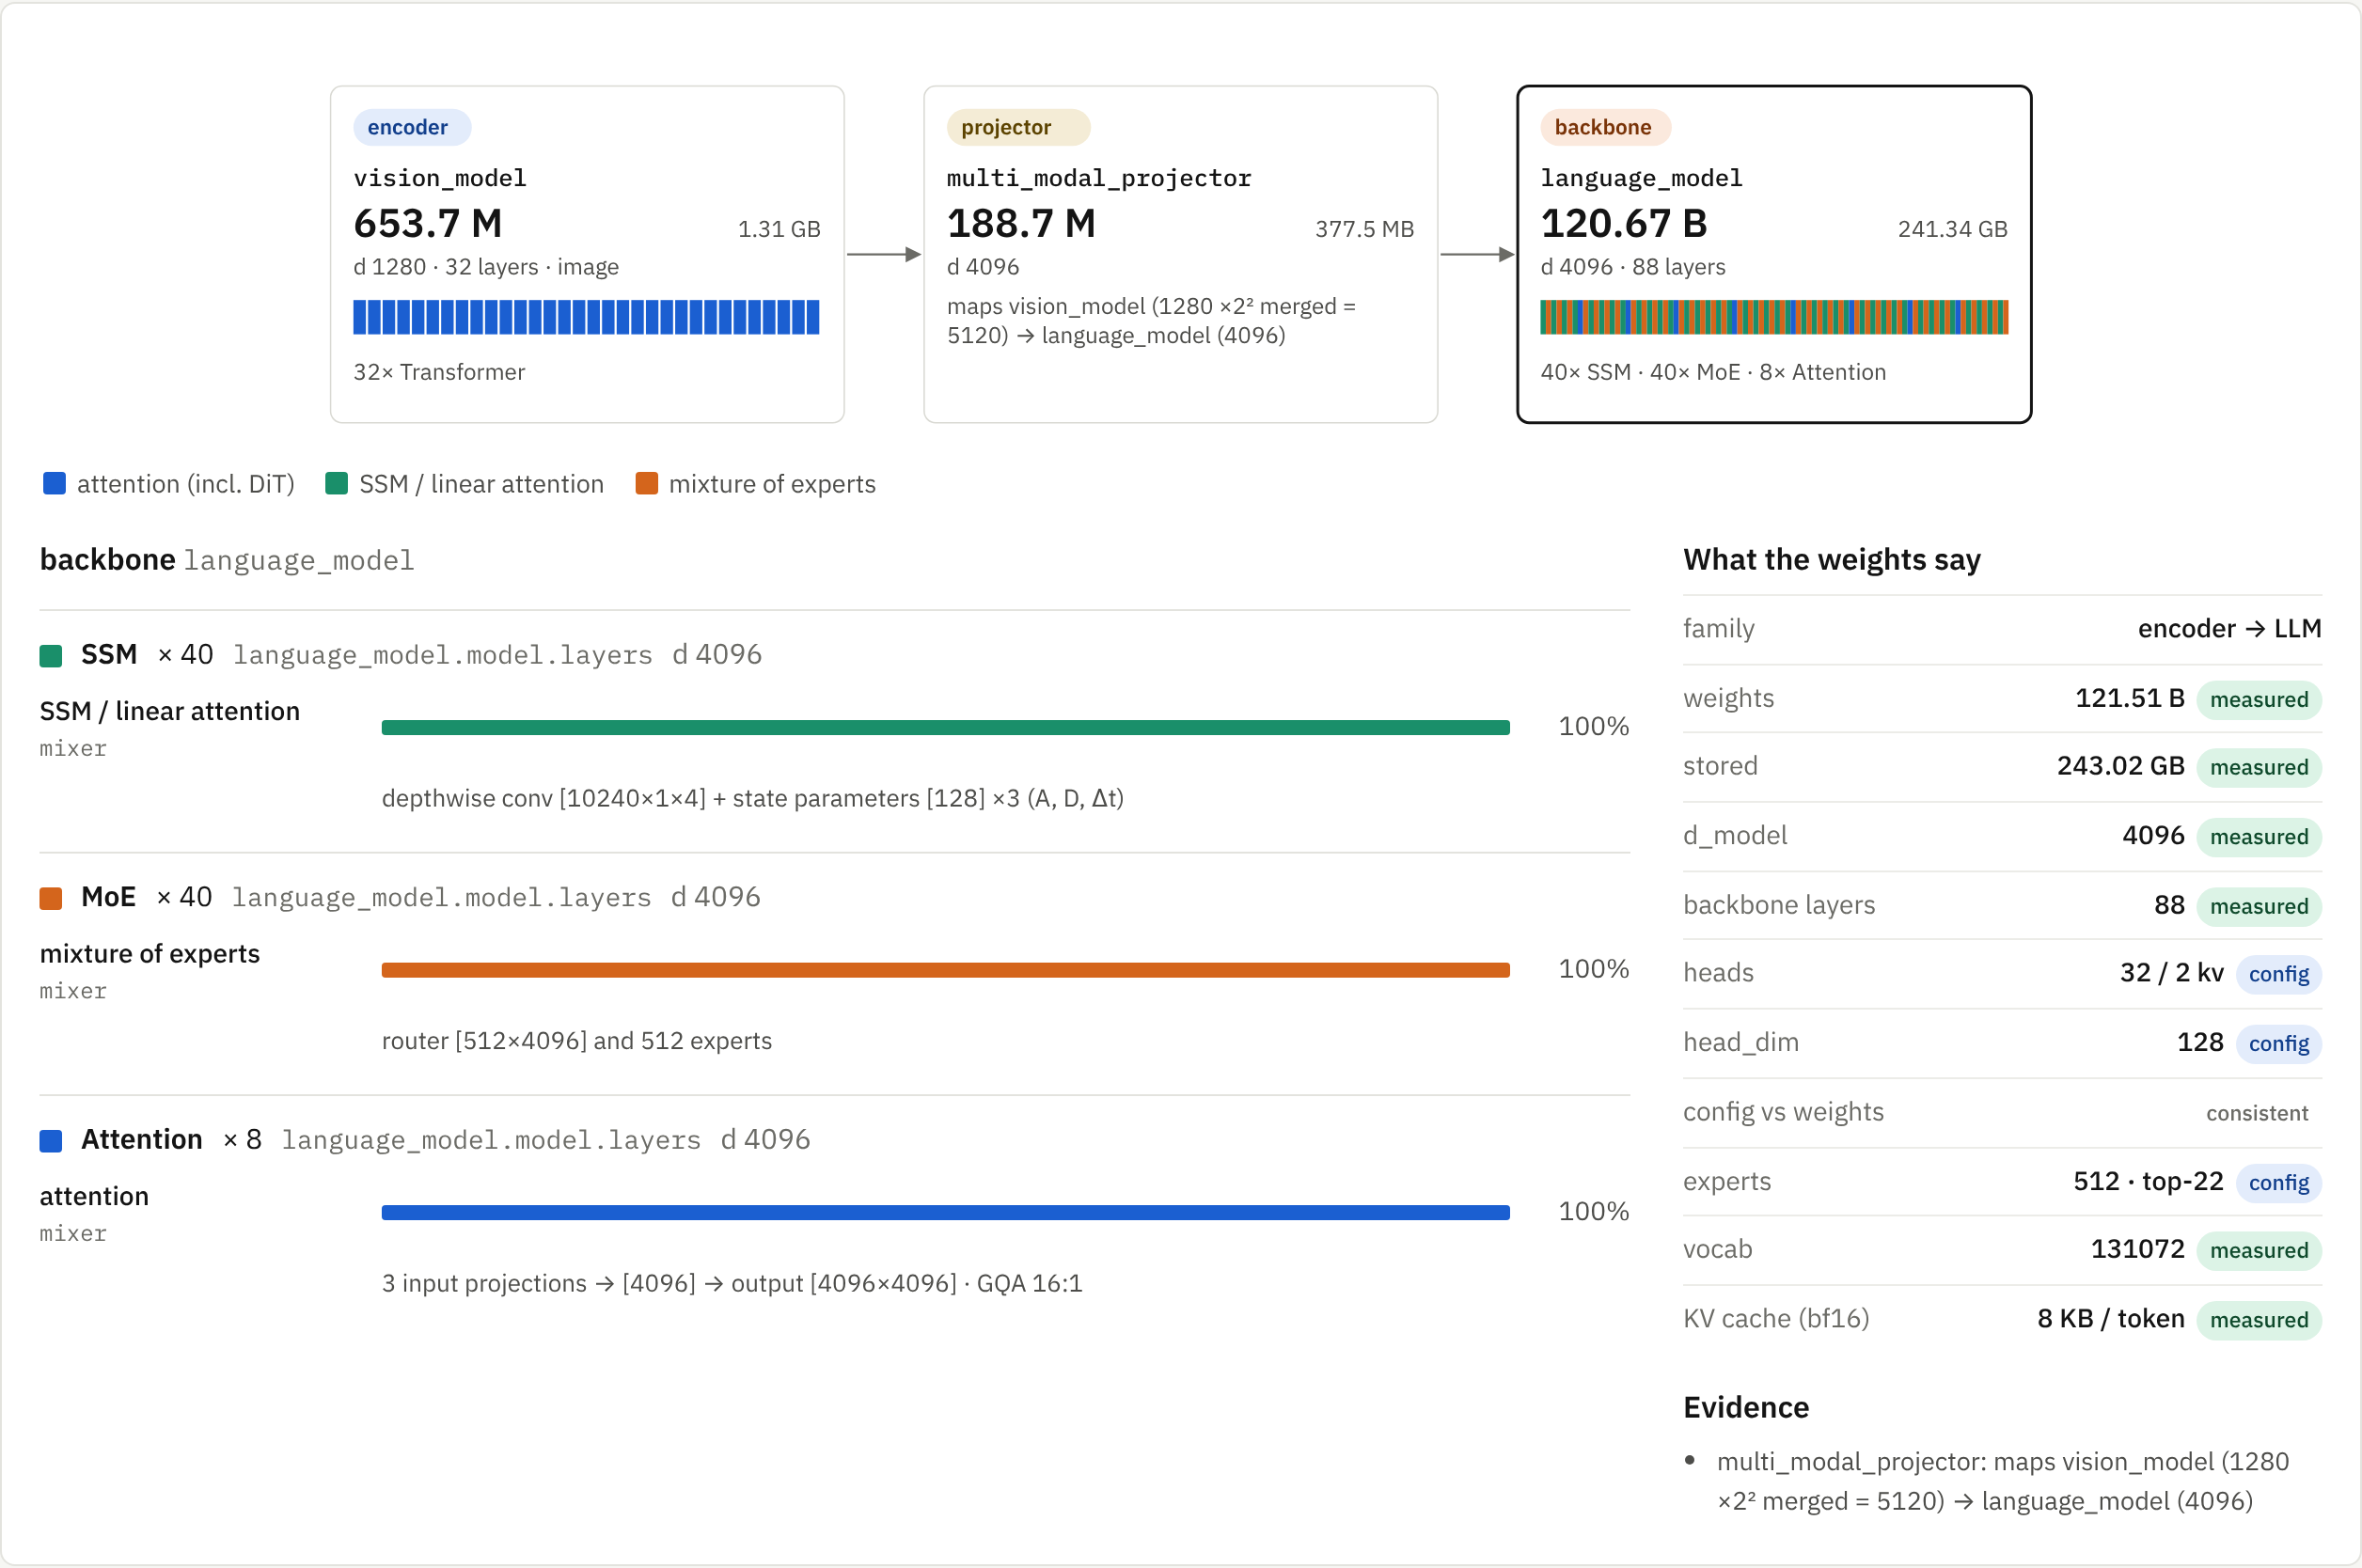
\includegraphics[width=\linewidth]{fig/ui_anatomy_supervl.png}
\caption{Anatomy view for Nemotron 3.5 Super VL (121.5\,B). Vision tower, projector and backbone in data-path order; the backbone's strip shows the interleaving of SSM (green), MoE (orange) and attention (blue) layers. Below, each block type with the share of parameters per region and the evidence behind its label; on the right, the values read from the model with their provenance and the result of the configuration check.}
\label{fig:ui-anatomy}
\end{figure}

\begin{figure}[t]
\centering
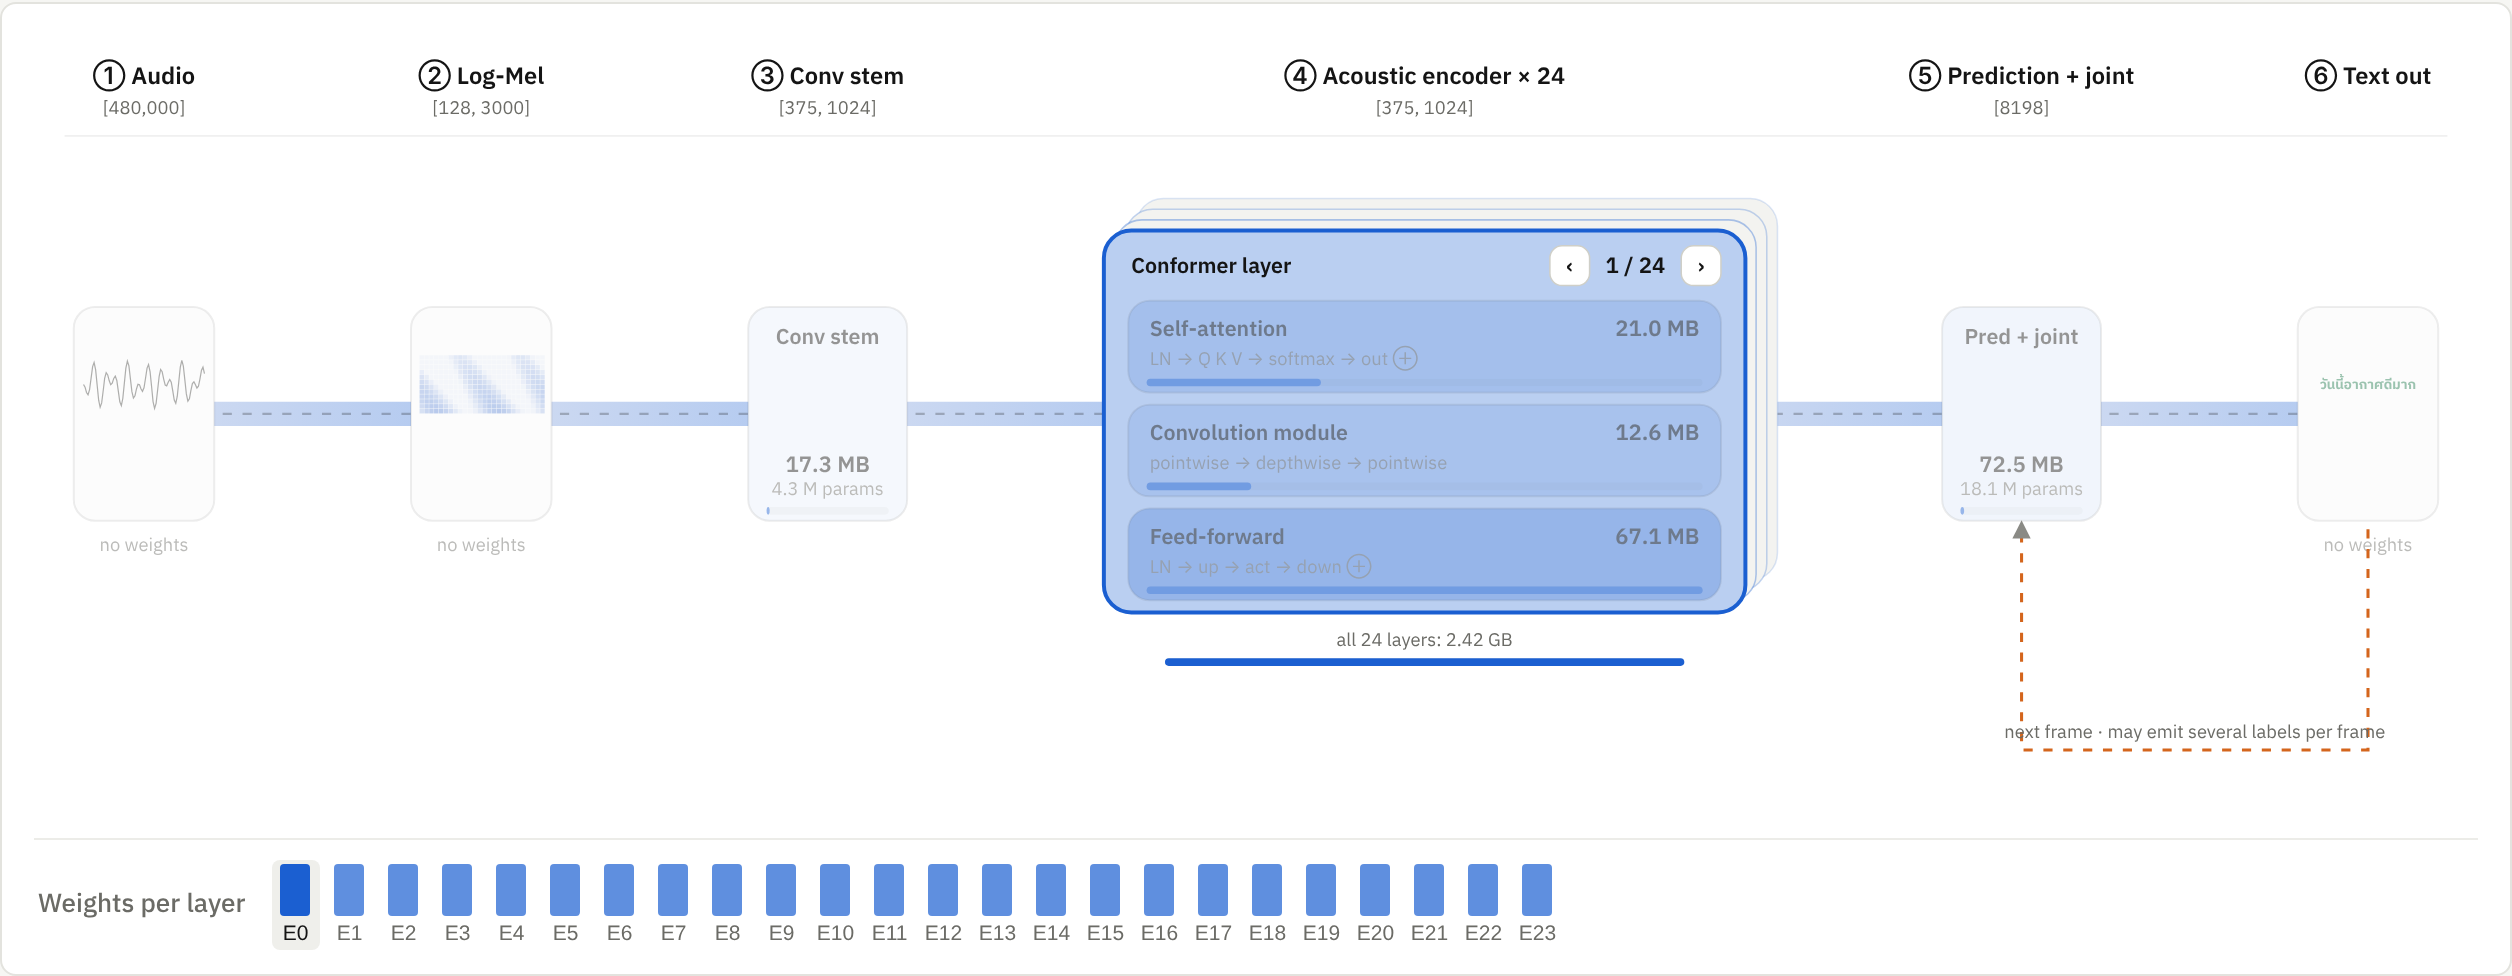
\includegraphics[width=\linewidth]{fig/ui_big_parakeet.png}\\[2pt]
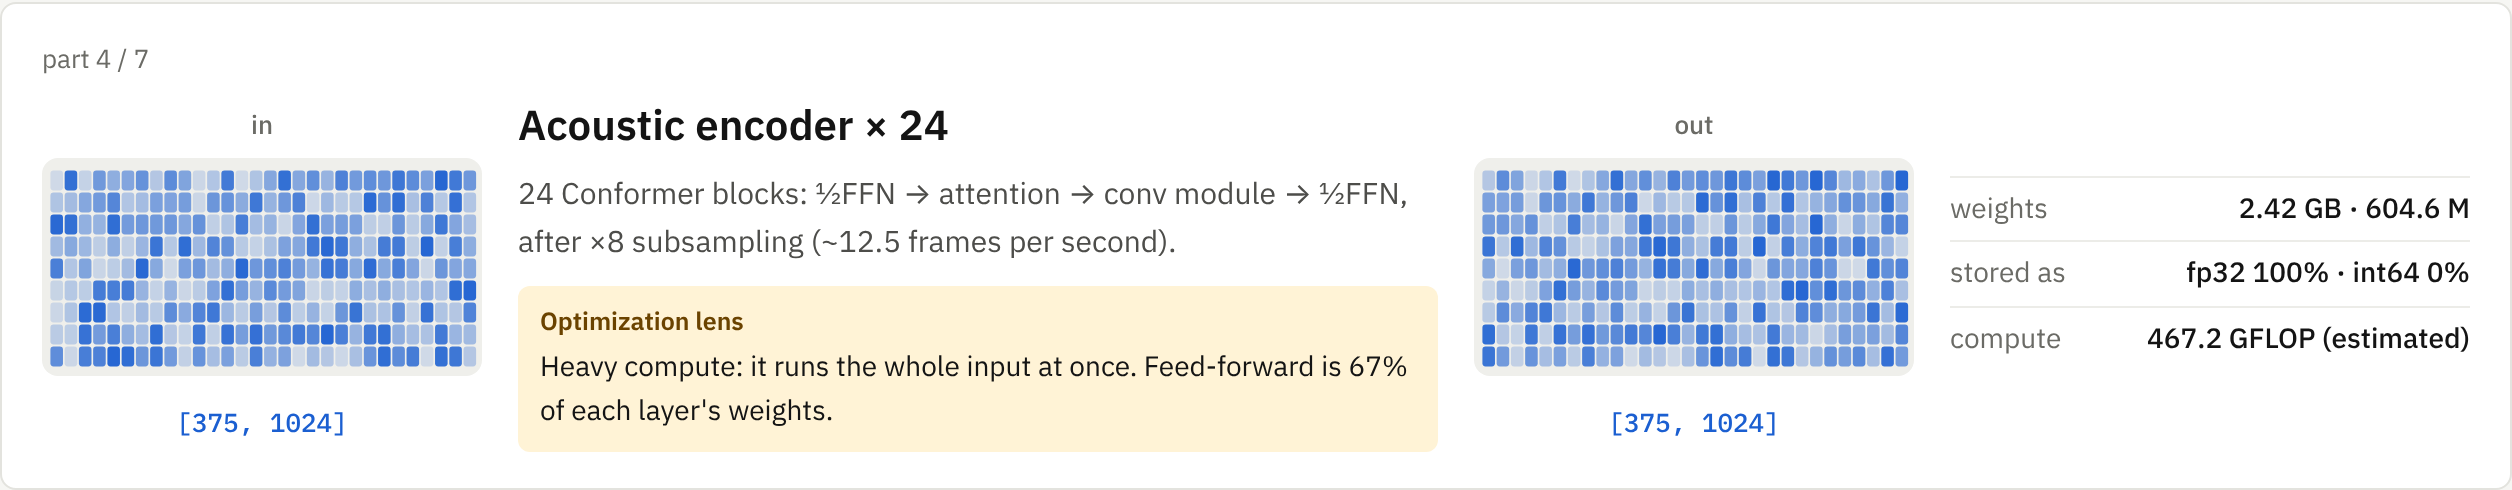
\includegraphics[width=\linewidth]{fig/ui_io_parakeet.png}
\caption{Big picture and play-through for Parakeet TDT 0.6B v3. Top: the transducer laid out from audio to text, with the prediction and joint networks as one part and the per-frame loop drawn back to them. Bottom: the panel for step 4 of 7, the acoustic encoder, with its input and output shapes, stored size, precision and estimated compute.}
\label{fig:ui-play}
\end{figure}

\paragraph{A usage walkthrough.} Suppose a user wants to deploy \tn{nvidia/parakeet-tdt-0.6b-v3} on a phone. They paste the repository id and press \emph{Load}. The explorer lists the repository, fetches \tn{config.json} and the 63\,KB header of the 2.5\,GB weight file, and finishes in well under a second on a normal connection. The anatomy view shows three components: a 24-block conformer encoder holding 97\% of the parameters, a 12\,M prediction network with a two-layer LSTM, and a 6\,M joint network whose output size, 8198, is the label vocabulary plus five duration bins. The block view shows that feed-forward modules hold two thirds of each conformer block, which suggests where pruning or low-bit storage pays. The play-through then explains that the encoder runs once per utterance, whereas the prediction and joint networks run per emitted label, so latency in streaming use is governed by the small networks, not by the encoder.

\paragraph{Implementation.} The tool is a single static page with no server component, about 3{,}000 lines of JavaScript, and runs offline once loaded. The recovery code is a separate module shared with the evaluation harness, so the benchmark measures exactly the code users run. Analysed models are stored in the browser's IndexedDB.

\section{Evaluation setup}
\label{sec:setup}

We ask five research questions.
\RQ{1} How accurately are per-tensor roles recovered, and how much depends on names?
\RQ{2} Are stacks, block counts and block types recovered?
\RQ{3} Is recovery robust to quantized storage?
\RQ{4} Which hyperparameters can shapes identify, how much does configuration fusion add, and do configurations agree with their weights?
\RQ{5} What does recovery cost?

\paragraph{Corpus.} \tn{transformers} 5.22.1~\citep{wolf2020transformers} registers 788 configuration types. For each, we instantiate the default configuration with the most specific model class available on PyTorch's meta device, which creates shapes without allocating memory. 548 types instantiate; removing identical manifests leaves 511. Tied parameters are counted once and persistent buffers are kept, as a saved checkpoint would. The corpus has 268{,}040 tensors (median 419 per model) and spans 1.5\,K to 1.74\,T parameters (median 473\,M). Of the 511 models, 475 contain attention, 73 mixtures of experts, 27 SSM or linear-attention mixers, 140 convolutional parts and 70 cross-attention; 231 have more than one stack and 153 have a stack with more than one block type. The configuration of each model is serialized with it for \RQ{4}.

\paragraph{Ground truth.} Labels come from information the algorithm never sees: the Python class of every module. A tensor's role is given by its nearest ancestor class whose name ends in a recognized suffix (\tn{Attention}, \tn{MLP}, \tn{SparseMoeBlock}, \tn{Mamba2Mixer}, \tn{RMSNorm}, \dots), with MoE containers overriding their children and a short list of module-name fallbacks for loose tensors; tensors that match nothing are labeled \emph{other} and excluded. Convolutional stems and position tables outside block stacks are merged into one \emph{input stem} role, because the library is inconsistent about which class owns them. Block lists are module lists whose children each hold at least two parameterized sub-modules, excluding expert containers and applying the same sub-layer convention as the algorithm; block types are the distinct class-composition signatures of the items. Hyperparameters come from the configuration, using the text sub-configuration for multimodal models.

\paragraph{Metrics.} Per-tensor role accuracy is weighted by parameter count within each model and averaged over models (\emph{macro}, our headline, so that every architecture counts once) or pooled over all tensors (\emph{micro}, which the largest models dominate). We also report per-role F1 over tensors; recall and precision of block lists by path; the share of matched lists with the exact block count and with the exact type partition; exact-match accuracy of hyperparameters; and exactness of the logical parameter total.

\paragraph{Conditions and baseline.} \emph{Names + shapes} is the full method. \emph{Shapes only} replaces every non-numeric path token by a consistent random hash, removing all lexical evidence while keeping the tree; it approximates checkpoints exported by unfamiliar code. \emph{Quantized} rewrites every 2-D linear weight as NVFP4 (group 16), FP8 with per-channel scales, or GPTQ 4-bit with group 128 (Appendix~\ref{app:quant}). The \emph{baseline} is a careful set of name-pattern rules of the kind most tools use, taken from the previous version of our own explorer: regular expressions for layer indices, \tn{q\_proj}/\tn{query}/\tn{c\_attn}, \tn{mlp}/\tn{fc1}/\tn{intermediate}, \tn{encoder\_attn}, \tn{mixer}, and so on.

\section{Results}
\label{sec:results}

\begin{table}[t]
\centering
\small
\begin{tabular}{lccccccc}
\toprule
& \multicolumn{2}{c}{Role accuracy (\%)} & \multicolumn{4}{c}{Block lists (\%)} & Params \\
\cmidrule(lr){2-3}\cmidrule(lr){4-7}
Condition & macro & micro & recall & precision & count & types & exact \\
\midrule
Names + shapes (ours) & \textbf{96.4} & \textbf{99.9} & 98.6 & 91.4 & 100 & 92.5 & 511/511 \\
Shapes only (ours) & 94.7 & 99.8 & 98.6 & 91.4 & 100 & 92.5 & 511/511 \\
Name patterns & 69.2 & 8.4 & -- & -- & -- & -- & -- \\
Name patterns, names hashed & 0.0 & 0.0 & -- & -- & -- & -- & -- \\
\midrule
Ours, NVFP4 storage & 96.4 & 99.9 & 98.6 & 91.4 & 100 & 92.5 & 511/511 \\
Ours, FP8 storage & 96.4 & 99.9 & 98.6 & 91.4 & 100 & 92.5 & 511/511 \\
Ours, GPTQ storage & 96.4 & 99.9 & 98.6 & 91.4 & 100 & 92.5 & 511/511 \\
Ours, shapes only + NVFP4 & 94.7 & 99.8 & 98.6 & 91.4 & 100 & 92.5 & 511/511 \\
\bottomrule
\end{tabular}
\caption{Main results on 511 architectures. \emph{count}: matched lists with the exact number of blocks; \emph{types}: matched lists whose block-type partition equals the ground truth. The name-pattern baseline produces no stacks. Micro accuracy is dominated by the three largest models, all trillion-parameter mixtures of experts, whose experts we label correctly and the baseline does not.}
\label{tab:main}
\end{table}

\subsection{\RQ{1}: Roles}
Per-tensor role accuracy is 96.4\% macro (Table~\ref{tab:main}). The distribution over models is skewed: the median model is labeled perfectly, 411 of 511 reach 99\% and 468 reach 90\%, while 10 fall below 50\%. Name-pattern rules reach 69.2\% macro; their micro accuracy collapses to 8.4\% because the corpus's parameter mass sits in a few trillion-parameter MoE defaults whose experts they mislabel. With names hashed the baseline has nothing to work with, whereas our method loses 1.7 points (371 models still reach 99\%). Most of the work is therefore done by structure and shapes, not vocabulary.

Figure~\ref{fig:f1} breaks the result down by role. Attention, feed-forward, MoE and norms exceed 96 F1 with names and stay above 91 without them. Cross-attention falls from 98 to 71 without names, which is expected: when encoder and decoder share a width, the two attention regions of a decoder block have identical shapes, and only a name says which reads the encoder. adaLN modulation (4 models) and recurrent cells (6 models) have too few examples for stable F1. Output heads score lowest, mostly because pooler and prediction-transform layers are labeled \emph{head} by the class oracle but look like a feed-forward or an embedding to the shape rules.

\begin{figure}[t]
\centering
\begin{minipage}[t]{.49\linewidth}\centering
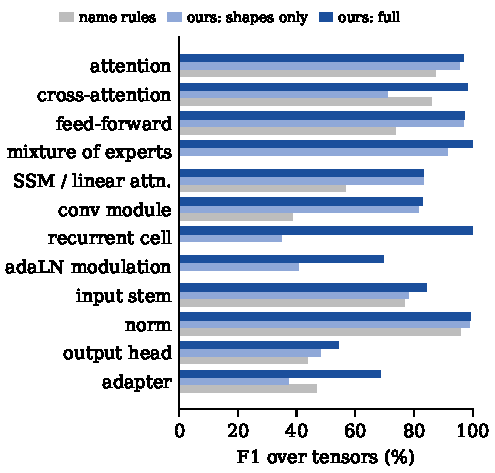
\includegraphics[width=\linewidth]{fig/f1_roles.pdf}
\caption{Per-role F1 over tensors.}
\label{fig:f1}
\end{minipage}\hfill
\begin{minipage}[t]{.49\linewidth}\centering
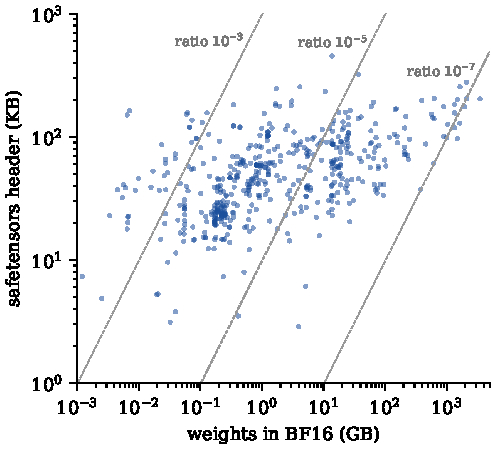
\includegraphics[width=\linewidth]{fig/header_cost.pdf}
\caption{Header size against weight size for the 511 manifests (one 3\,KB model lies off the left edge). Dashed lines mark constant ratios; the median header is 47\,KB and the largest 453\,KB.}
\label{fig:cost}
\end{minipage}
\end{figure}

The largest error groups are informative. ConvBERT's span-based dynamic convolution sits inside its attention module, so the region is labeled a convolution. The linear-attention layers of GLM-5-Next keep ordinary query, key and value projections and move the decay parameters into a sub-module, so the shape rules see attention; the opposite happens in EdgeTAM's perceiver, whose gated attention looks recurrent. ALBERT shares one layer across depth and stores no list at all. I-BERT keeps integer copies of every weight whose matching shapes imitate a gate stack, which also produces the only false transducer detection in the corpus; the three real transducers are found. The ten models below 50\% (ALBERT, I-BERT, xLSTM, XLNet, MobileBERT, MobileViTv2, PoolFormer, PatchTSMixer, NeoMME and an ASR encoder with fused blocks) each depart from the block conventions the rules assume rather than failing on a common architecture.

\subsection{\RQ{2}: Stacks and block types}
98.6\% of ground-truth block lists (1232 of 1250) are found at the right path, and every matched list has the right number of blocks. Precision is lower (91.4\%) because the algorithm also reports repeated sub-blocks inside convolutional backbones, such as ResNet bottleneck sub-layers and SEANet residual units, that the ground-truth convention does not count. The block-type partition is exact for 92.5\% of matched lists; most misses are lists whose first block differs only in a module the class signature sees and the tensor signature does not, such as a relative-position bias owned by layer 0.

\subsection{\RQ{3}: Quantized storage}
Under NVFP4, FP8 and GPTQ storage the results equal those at full precision, and logical parameter totals remain exact for all 511 models (Table~\ref{tab:main}). This holds with names hashed as well, because packed weights and their scales are recognized by dtype and shape ratios rather than by suffixes such as \tn{weight\_scale}. The point has practical weight: hub pages count packed bytes as parameters, so an NVFP4 model is often displayed at about 60\% of its real size (\S\ref{sec:cases}).

\subsection{\RQ{4}: Identifiability, configuration fusion and consistency}
\label{sec:rq4}

\begin{table}[t]
\centering
\small
\begin{tabular}{lcccccccc}
\toprule
& $d$ & layers & FFN & experts & vocab & heads & KV heads & head size \\
\midrule
Manifest only, all models & 92.7 & 92.1 & 90.5 & 97.3 & 87.2 & 72.2 & 70.0 & 66.7 \\
\quad $n$ & 468 & 442 & 336 & 74 & 360 & 446 & 227 & 153 \\
Manifest only, single stack & 95.0 & 96.3 & 94.1 & 96.4 & 85.6 & 70.3 & 63.9 & 57.1 \\
Manifest only, shapes only & 92.7 & 92.1 & 90.5 & 94.6 & 84.7 & 72.2 & 70.0 & 66.7 \\
With configuration fusion & -- & -- & -- & -- & -- & 96.0 & 98.2 & 96.7 \\
\midrule
Identifiable from shapes? & yes & yes & yes & yes & yes & \multicolumn{3}{c}{only with per-head parameters} \\
\bottomrule
\end{tabular}
\caption{Exact-match accuracy (\%) of hyperparameters against the configuration. FFN is evaluated on dense models only. Fusion is evaluated on the 510 models whose configuration serialized.}
\label{tab:hp}
\end{table}

Table~\ref{tab:hp} separates identifiable from non-identifiable fields. Width, depth, FFN size and expert count are read correctly for 90--97\% of models, and more often when a model has a single stack, which removes ambiguity about which component the configuration describes. From shapes alone, head count and head size are right about 70\% of the time. The prior is right more often (78\%) than a norm vector of plausible length (69\%): in latent attention, the norm before the low-rank KV projection has the latent width, not the head width. This is a concrete instance of the identifiability limit of \S\ref{sec:ident}.

With configuration fusion, head count, KV head count and head size are right for 96.0\%, 98.2\% and 96.7\% of models. Because the ground truth comes from the same configuration, this number measures the \emph{matching} step, that is, whether the right sub-configuration is attached to the backbone, rather than independent accuracy; the backbone found a match in 456 of 510 models and 874 of 1108 components found one. The more informative result is the consistency check. Of the 635 matched components with attention, 603 (95.0\%) have configurations whose head fields multiply out to the projection widths in the weights. The 32 disagreements are concentrated in latent-attention models (DeepSeek-V2/V3/V4, Kimi, MiniCPM3, Mistral 4, LongCat-Flash), where \tn{head\_dim} or \tn{num\_key\_value\_heads} refers to the query--key or latent geometry rather than to a projection width, in Falcon's fused multi-query layout, and in SAM-style windowed vision encoders. None of them is a wrong configuration; each is a field whose meaning is family-specific. A tool that silently trusted the configuration would report wrong KV-cache sizes for exactly these models, which is why the explorer shows the mismatch instead of resolving it.

\subsection{\RQ{5}: Cost}
The median safetensors header is 47\,KB, the 95th percentile 164\,KB and the largest 453\,KB, for models up to 3.5\,TB in BF16 (Figure~\ref{fig:cost}). Recovery takes 12.6\,ms for the median model in a single JavaScript thread (95th percentile 63\,ms, maximum 177\,ms). In the explorer, network round trips dominate: a single-file model needs four requests (listing, configuration, two range requests), and a sharded model two range requests per shard.

\section{Case studies: nine models from 2026}
\label{sec:cases}

\begin{table}[t]
\centering
\footnotesize
\setlength{\tabcolsep}{4pt}
\begin{tabular}{p{3.3cm}p{1.6cm}rrp{6.2cm}}
\toprule
Model & Family & Params & Header & Recovered anatomy (selected) \\
\midrule
Nemotron 3.5 Super VL 120B-A12B & prefix LM & 121.5\,B & 130\,KB & ViT tower (32 L, $d$ 1280) $\to$ projector $1280{\times}2^2{=}5120\to20480\to4096$ $\to$ 88-layer backbone: 40 SSM, 40 MoE (512 experts, 92.8\% of weights), 8 attention (2 KV heads, 8\,KB KV per token) \\
Nemotron 3.5 Transcribe 30B-A4B & prefix LM & 32.4\,B & 154\,KB & audio encoder (32 L, $d$ 1280), diarization encoder (31 L, $d$ 512), word-timestamp encoder, projector $1280\to2688$, 52-layer backbone: 23 SSM, 23 MoE (128 experts), 6 attention; 4.36\,B active with top-6 \\
Nemotron 3.5 ASR streaming 0.6B & transducer & 638\,M & 57\,KB & 24 conformer blocks; LSTM prediction net; joint $1024,640\to640\to13088$, no duration bins (RNN-T) \\
Parakeet TDT 0.6B v3 & transducer & 627\,M & 63\,KB & same encoder shape; joint output $8198=8193+5$ duration bins (TDT); total within 24 of the hub's figure \\
Nemotron 3 Embed 1B NVFP4 & encoder & 1.14\,B & 41\,KB & 16 blocks, $d$ 2048, 24/8 heads (config, consistent), 112 NVFP4 linear layers (group 16), tied table; stored 1.03\,GB \\
FastH3 Omni FP8 (transformer)$^\dagger$ & diffusion & 33.1\,B & 84\,KB & 2 refiner + 50 DiT blocks, 56 heads of 128 (measured from $q$/$k$ norms), adaLN $18d$ (6 terms $\times$ 3 modalities), timestep MLP $256\to5376\to2688$; 300 FP8 tensors, 47.0 vs.\ 66.3\,GB \\
Kumo Tabular (large)$^\dagger$ & encoder & 214\,M & 41\,KB & row embedding (6 induced + 6 row blocks, $d$ 256) and 24-layer ICL backbone ($d$ 1024); 854\,MB in FP32 vs.\ 855\,MB file \\
Kumo Relational$^\dagger$ & encoder & 29\,M & 24\,KB & row embedding $\to$ message passing (4 square maps, 5 reducers) $\to$ 12-layer ICL backbone; 118 vs.\ 120\,MB file \\
\bottomrule
\end{tabular}
\caption{Anatomies recovered for 2026 models (the BF16 FastH3 variant gives the same structure). Manifests marked $^\dagger$ are rebuilt from public source code and configuration because no reference implementation is in \tn{transformers}; the others are generated from the published \tn{config.json} by the reference implementation, with NVFP4 storage following the published quantization config.}
\label{tab:cases}
\end{table}

These models were not in the benchmark, but they were not held out from development either: we studied them while extending the rules, and several parts of \S\ref{sec:method} (transducer joints, timestep MLPs, message-passing layers, adapter components) were written because of them. Every change was checked on the full benchmark for regressions. The case studies therefore show that the representation is rich enough for these architectures; the unbiased accuracy estimate is \S\ref{sec:results}. Table~\ref{tab:cases} summarizes them.

\paragraph{A 121B hybrid.} The Super VL backbone mixes three block types in one list, and the recovered type sequence reproduces the configuration's \tn{layers\_block\_type} exactly. The projector's input width, 5120, is four times the vision width; the algorithm reports a $2\times2$ merge, which matches the configuration's \tn{downsample\_ratio} of 0.5. Experts hold 112.7\,B of 121.5\,B parameters. With the configured top-22 routing that gives 13.6\,B active parameters per token, including the vision tower and both embedding tables, against the 12\,B in the model's name. Only 8 of 88 layers keep a KV cache, each with 2 KV heads, so the cache costs 8\,KB per token in BF16; if all 88 layers used the same attention it would be eleven times larger.

\paragraph{Transducers.} For both speech models the joint network is found from three shapes, and the number of duration bins falls out as a difference: Parakeet's joint output has 8198 rows and its label table 8193, giving the five durations $\{0,\dots,4\}$ of its configuration, while the streaming model's two sizes are equal (a standard RNN-T). Parakeet's parameter total differs from the hub's by 24, the number of batch-norm step counters, one per conformer block.

\paragraph{Packed weights and encoders.} The NVFP4 embedding model has 1.14\,B logical parameters, matching its model card, while the hub's file statistics report 0.7\,B because they count packed \tn{U8} elements. That it is an encoder cannot be seen in the weights; its configuration's \tn{is\_causal: false} settles it, and the explorer labels the family as coming from the configuration.

\paragraph{What the case studies taught us.} Besides the new components, four fixes to existing rules came from these models: the residual width of a block is taken from its norms; \tn{nn.Sequential} children are no longer split as sub-layers; a module wrapping two different sub-blocks is split; and in repositories with several top-level folders, homes are not raised above the folder. The streaming ASR model's language-prompt projector remains unattached, because its prompt table lives outside the manifest's components.

\section{Discussion and limitations}
\label{sec:limits}

\paragraph{Ground truth.} Class names are an independent signal but not a perfect one. Some implementations place a position table inside a class called \tn{...Embeddings} and others inside the encoder; some call a pooler a \tn{...Head}. We merged roles where the library is inconsistent and kept the fallback list short, but per-role numbers for heads and adapters should be read with this in mind. The headline numbers are robust to it because these roles carry little parameter mass.

\paragraph{One library's conventions.} All corpus manifests come from \tn{transformers} implementations, which share naming habits. The shapes-only condition is the main protection against overfitting to those habits, and its 1.7-point drop suggests the structural rules transfer. Default configurations are not trained checkpoints, but their shapes, which are all the method reads, are the same as those of trained ones.

\paragraph{Configuration fusion.} Fusion accuracy is measured against the same configuration that supplies the fields, so it validates the matching step, not the configuration. The consistency check is the independent part, and its disagreements point at fields whose meaning differs by family; a richer check could model latent attention explicitly.

\paragraph{Reconstructed manifests and scope.} Three case-study manifests were rebuilt from source; their totals match the published file sizes within 2\%, but module prefixes in the real checkpoints may differ. The explorer reads the real headers when given a repository. GGUF and ONNX files are not handled yet, although both carry comparable metadata; old non-zip PyTorch pickles are rejected. Order inside a block and activation functions remain unknown, and FLOP estimates assume standard computation per role.

\paragraph{Responsible use.} The method reads only what a hub already serves publicly. It never downloads or executes weights, and the PyTorch reader interprets a fixed subset of pickle opcodes as data without resolving Python callables.

\section{Conclusion}

A tensor manifest is small, safe and almost always available, and it carries more of an architecture than one might expect. With the module tree, a few dozen shape rules and width matching, we recover blocks, block types, regions, data paths and logical sizes for 511 architectures at 96\% role accuracy, keep most of that accuracy without any names, and stay exact on parameter counts under modern quantized formats. The same analysis makes the limits explicit: head geometry, masking and routing are not in the shapes. Fusing them from the configuration closes most of the gap, and checking the configuration against the weights exposes the families whose fields mean something else. We hope the benchmark and the explorer make it routine to look inside a model before downloading it.

\paragraph{Availability.}\sloppy The explorer runs at \url{https://joessattes.github.io/ai-model-explorer/}. Source code, the corpus builder, the evaluation harness and this paper's sources are at \url{https://github.com/JoesSattes/ai-model-explorer} under the MIT license. The results in \S\ref{sec:results} are reproduced by \tn{python research/build\_corpus.py corpus.jsonl} followed by \tn{node research/eval.js corpus.jsonl} with the flags \tn{--obf --nolex}, \tn{--quant nvfp4|fp8|gptq}, \tn{--v1} and \tn{--cfg}.

\bibliographystyle{plainnat}
\bibliography{refs}

\appendix
\section{Corpus construction details}
The model class for each configuration type is chosen in this order: image-text-to-text, multimodal LM, speech sequence-to-sequence, sequence-to-sequence LM, TDT, RNN-T, causal LM, CTC, masked LM, image classification, text-to-waveform, object detection, base model. Instantiation uses \tn{\_from\_config} under \tn{torch.device("meta")} with a 90-second limit. Of the 240 types that do not instantiate, 177 are sub-configurations without a model class of their own (vision or audio towers registered separately), and the rest fail on required sub-configurations or optional dependencies. Manifests are deduplicated by the exact list of names and shapes.

\section{Synthetic quantized storage}
\label{app:quant}
For every 2-D tensor named \tn{*.weight} whose input dimension is a multiple of 32 and output dimension a multiple of 8, excluding embeddings, heads and norms: NVFP4 replaces $[o,i]$ by \tn{U8} $[o,i/2]$, \tn{F8\_E4M3} $[o,i/16]$ and two \tn{F32} scalars; FP8 by \tn{F8\_E4M3} $[o,i]$ and \tn{F32} $[o,1]$; GPTQ by \tn{qweight} \tn{I32} $[i/8,o]$, \tn{qzeros} $[i/128,o/8]$, \tn{scales} \tn{F16} $[i/128,o]$ and \tn{g\_idx} $[i]$. Under name hashing these suffixes are hashed too, so recognition relies on dtypes and shape ratios.

\section{Additional interface views}
\begin{figure}[h]
\centering
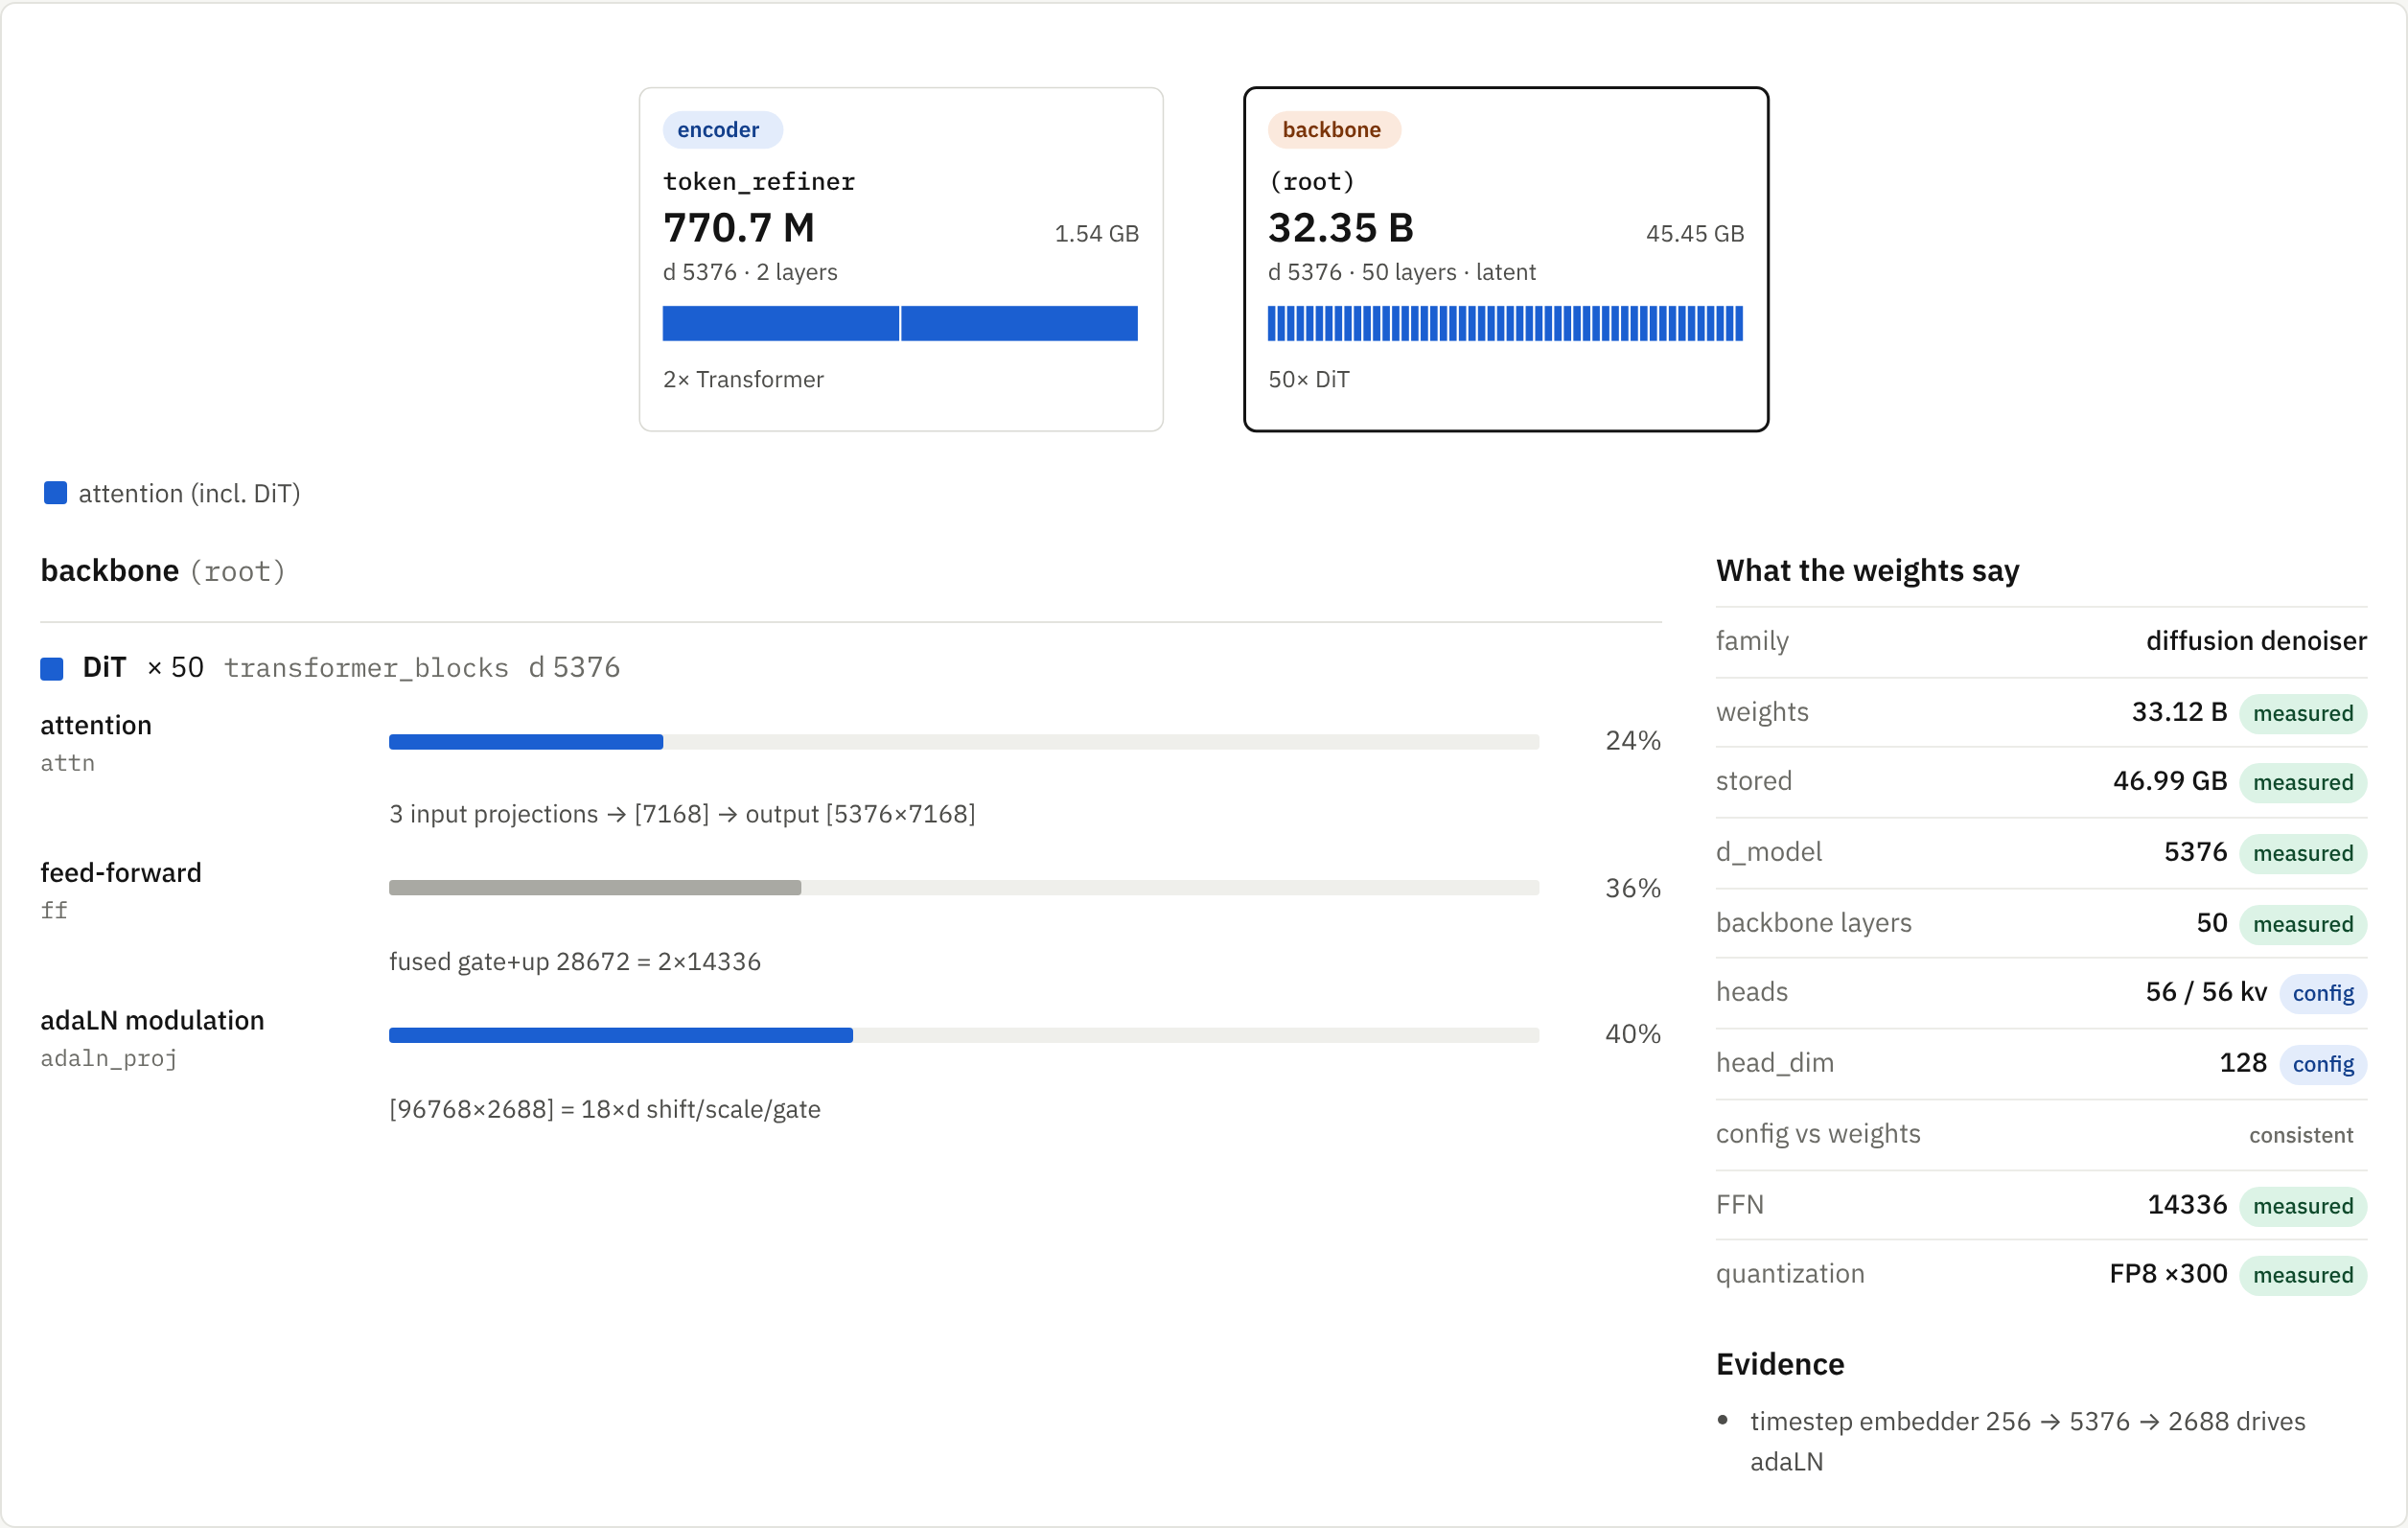
\includegraphics[width=\linewidth]{fig/ui_anatomy_fasth3.png}
\caption{Anatomy view for the FastH3 Omni FP8 denoiser (reconstructed manifest): a two-block token refiner and a 50-block DiT backbone. The head geometry is \emph{measured} from per-head norms, and the FP8 storage of 300 tensors is reported with logical and stored sizes.}
\end{figure}

\end{document}
